\chapter{More on Tree}

\section{Tries}
\subsection{Definition}
A trie, also called a digital tree, radix tree, or prefix tree, is a special type of tree used to store associative data structures. The name trie comes from its use for re\textbf{trie}val, because the trie can find a single word in a dictionary with only a prefix of the word. 

For example, strings are stored in a top-to-bottom manner based on their prefixes in a trie. All prefixes of length 1 are stored at level 1, all prefixes of length 2 are stored at level 2, and so on. For the string set \( S = \{ \text{bear}, \text{bell}, \text{bid}, \text{bull}, \text{but}, \text{sell}, \text{stock}, \text{stop} \} \), we can have:
\begin{figure}[H]
  \centering
  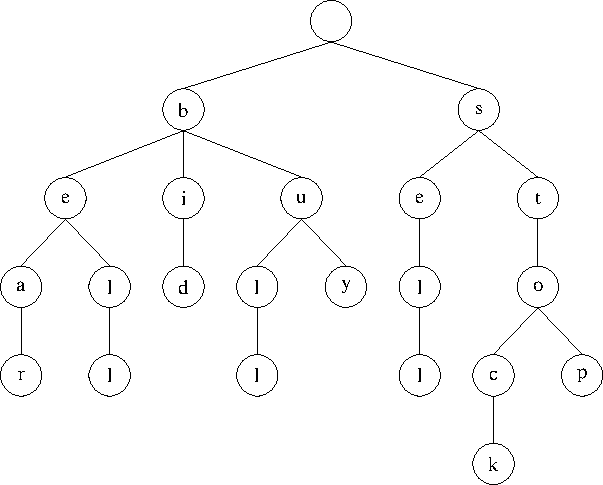
\includegraphics[width=0.5\textwidth]{Figure/Tries.pdf}  
\end{figure}
This figure shows how the strings are stored in the trie. Inserting and deleting words in this tree is straightforward. For example, when typing "belt," it can be inserted in the subtree starting from \verb|b -> e -> l|.

Unlike a binary search tree, no node in a trie stores the key associated with that node; instead, its position in the tree defines the key with which it is associated. 

All the descendants of a node share a common prefix in the string associated with that node, and the root is associated with the empty string.

\subsection{Advantages}
A trie can also be used to replace a hash table, offering the following advantages:

1. Faster lookup: Looking up data in a trie is faster than the worst case of a hash table. For a trie, the time complexity is \(O(m)\), where \(m\) is the length of the search string. However, the time for an imperfect hash table would be \(O(n)\), where \(n\) is the total number of strings.

2. No collisions: There are no collisions of different keys in a trie, unlike hash tables, where collisions can occur when two keys map to the same hash value.

3. No need for a hash function: In a trie, there is no need to provide a hash function or change it as more keys are added, unlike hash tables that require such adjustments.

4. Alphabetical ordering: A trie can provide an alphabetical ordering of the entries by key, making it useful for applications like autocomplete or lexicographical ordering.

\subsection{Applications}
A common application of a trie is storing a predictive text or autocomplete dictionary, such as those found on mobile phones. It is also used in web browsers, which autocomplete your text or show possible completions for the text you are typing. Additionally, a trie can act as an orthographic corrector, checking whether every word you type exists in a dictionary.

\subsection{Analysis}
A standard trie uses \(O(n)\) space and supports searches, insertions, and deletions in time \(O(dm)\), where \(n\) is the total size of the strings in \(S\), \(m\) is the size of the string parameter of the operation, and \(d\) is the size of the alphabet.
